\section{Analizando el Algoritmo}

Para analizar el algoritmo propuesto anteriormente, va a resultar útil plantear un ejemplo para analizar el comportamiento:
Sea el arreglo de monedas $A = [96. 594, 437, 674, 950]$.
Creamos la tabla o matriz para poder ir anotando los optimos, ademas la llenamos de ceros.

\begin{table}[!ht]
    \centering
    \begin{tabular}{|l|l|l|l|l|l|}
    \hline
        indices & 0 & 1 & 2 & 3 & 4 \\ \hline
        0 & 0 & 0 & 0 & 0 & 0 \\ \hline
        1 & 0 & 0 & 0 & 0 & 0 \\ \hline
        2 & 0 & 0 & 0 & 0 & 0 \\ \hline
        3 & 0 & 0 & 0 & 0 & 0 \\ \hline
        4 & 0 & 0 & 0 & 0 & 0 \\ \hline
    \end{tabular}
\end{table}
\begin{itemize}
    \item Una vez esta la matriz creada, vamos recorriendo cada moneda, la moneda $0$ ira en la posicion $(0, 0)$, la moneda $1$ en la posición $(1, 1)$ y asi sucesivamente.
    \item Además, una vez tengamos la moneda $i$, en todos los pasos (excepto el final), vamos a comparar la moneda $i$ con su siguiente, o sea $i+1$, para asi ubicar la mayor de estas en la posicion $(i+1)$
\end{itemize}
\begin{table}[!ht]
    \centering
    \begin{tabular}{|l|l|l|l|l|l|}
    \hline
        indices & 0 & 1 & 2 & 3 & 4 \\ \hline
        0 & 96 & 594 & 0 & 0 & 0 \\ \hline
        1 & 0 & 594 & 594 & 0 & 0 \\ \hline
        2 & 0 & 0 & 437 & 674 & 0 \\ \hline
        3 & 0 & 0 & 0 & 674 & 950 \\ \hline
        4 & 0 & 0 & 0 & 0 & 950 \\ \hline
    \end{tabular}
\end{table}
\begin{itemize}
    \item En este caso podemos observar como para $i = 0$, en la posición $(0, 1)$ ubicamos al $594$, ya que el mismo es mas grande que su anterior, el $96$. Este mismo paso con todos las monedas (menos la ultima).
    \item Una vez tenemos la primer parte hecha, se prosigue a la segunda, donde hay que aplicar la ecuación de recurrencia. Al ser un algoritmo del tipo bottom-up (iterativamente), vamos a ir resolviendo el problema grande arrancando por los problemas mas chicos, esos empiezan utilizando unicamente tres monedas.
    \item Iniciamos con los subproblemas. Tenemos tres monedas y las mismas son $[96, 594, 437]$, ademas tenemos que $i = 0$ y $j = 2$. Primero evaluamos la ganancia que podriamos llegar a tener si elegimos la moneda de la izquierda, esta se compone de elegir el $96$ y saber que Mateo eligirá la mas grande entre $[594, 437]$, por lo que nos quedaria como ganancia izquierda = $96 + 437$, o lo que es lo mismo, $96 + OPT[0+2][2]$.
    \item Por otro lado, la ganancia derecha sera el resultado de tomar la ultima moneda, de valor $437$, por lo que mateo se que eligira la mayor entre $[594, 96]$ quedando nuevamente $437 + 96$, o $437 + OPT[0][2-2]$. Siendo que entonces el máximo aca es igual en ambos casos.
\end{itemize}
\begin{table}[!ht]
    \centering
    \begin{tabular}{|l|l|l|l|l|l|}
    \hline
        indices & 0 & 1 & 2 & 3 & 4 \\ \hline
        0 & 96 & 594 & 533 & 0 & 0 \\ \hline
        1 & 0 & 594 & 594 & 0 & 0 \\ \hline
        2 & 0 & 0 & 437 & 674 & 0 \\ \hline
        3 & 0 & 0 & 0 & 674 & 950 \\ \hline
        4 & 0 & 0 & 0 & 0 & 950 \\ \hline
    \end{tabular}
\end{table}
\begin{itemize}
    \item La distancia entre $i$ y $j$ sigue siendo de $3$, pero ahora $i = 1$ y $j = 3$. Con esos datos analizamos la lista que contiene a $[594, 437, 674]$, inicialmente elegimos a $597$, y Mateo va a elegir $674$, por lo que hacemos $594 + OPT[1+1][3-1]$ (o sea $437$), quedando una \textit{ganancia izquierda} de $1031$.
    \item Yendo hacia el final ahora, elegimos 674, Mateo eligirá $594$ por ser mas grande que $437$, entonces se vuelve a sumar $674 + OPT[1+1][2-1]$ ($437$), quedando una \textit{ganancia derecha} de $1111$ puntos. Siendo que entonces entre estos dos, Sophia va a elegir los $1111$ puntos en la posicion $OPT[1][3]$.
\end{itemize}
\begin{table}[!ht]
    \centering
    \begin{tabular}{|l|l|l|l|l|l|}
    \hline
        indices & 0 & 1 & 2 & 3 & 4 \\ \hline
        0 & 96 & 594 & 533 & 0 & 0 \\ \hline
        1 & 0 & 594 & 594 & 1111 & 0 \\ \hline
        2 & 0 & 0 & 437 & 674 & 0 \\ \hline
        3 & 0 & 0 & 0 & 674 & 950 \\ \hline
        4 & 0 & 0 & 0 & 0 & 950 \\ \hline
    \end{tabular}
\end{table}
\begin{itemize}
    \item Ahora $i = 2$ y $j = 4$, con la siguiente lista como material $[437, 674, 950]$. Tomando el elemento de la izquierda tenemos que, como Mateo tomara el $950$ por sobre el $674$, nos queda $437 + OPT[2+1][4-1]$ ($674$), siendo igual a $1111$.
    \item Por el otro lado, si tomamos la ultima, o sea la moneda de valor $950$, nos queda que, como Mateo tomara la de 674, sumamos $950 + OPT[2][4-2]$ ($437$) siendo igual a $1387$. Tomando como máximo entre la ganancia por izquierda y por derecha, a la ganancia por derecha, guardando ese valor en $OPT[2][4]$
\end{itemize}
\begin{table}[!ht]
    \centering
    \begin{tabular}{|l|l|l|l|l|l|}
    \hline
        indices & 0 & 1 & 2 & 3 & 4 \\ \hline
        0 & 96 & 594 & 533 & 0 & 0 \\ \hline
        1 & 0 & 594 & 594 & 1111 & 0 \\ \hline
        2 & 0 & 0 & 437 & 674 & 1387 \\ \hline
        3 & 0 & 0 & 0 & 674 & 950 \\ \hline
        4 & 0 & 0 & 0 & 0 & 950 \\ \hline
    \end{tabular}
\end{table}
\begin{itemize}
    \item Ahora si, el tamaño del subproblema crece, $i$ pasa a estar a $3$ numeros de $j$, por lo cual arrancamos con $i = 0$ y $j = 3$. Teniendo para trabajar la lista de $[96, 594, 437, 674]$. Si elegimos el $96$, sabremos que Mateo va a elegir entre el $594$ y el $674$, manteniendo su decisión avariciosa de agarrar el $674$, quedándonos $96 + OPT[0+1][3-1]$ ($594$) dando como \textit{ganancia izquierda} $690$ puntos.
    \item Del otro lado, tomando $674$, Mateo va a elegir $437$ por sobre $96$, por lo que nos queda como \textit{ganancia derecha} la cuenta de $674 + OPT[0][3-2]$ ($594$) siendo esto igual a $1268$ puntos. Y como además es mayor al resultado anterior, nos quedaremos con esta opcion, alojandola en $OPT[0][3]$.
\end{itemize}
\begin{table}[!ht]
    \centering
    \begin{tabular}{|l|l|l|l|l|l|}
    \hline
        indices & 0 & 1 & 2 & 3 & 4 \\ \hline
        0 & 96 & 594 & 533 & 1268 & 0 \\ \hline
        1 & 0 & 594 & 594 & 1111 & 0 \\ \hline
        2 & 0 & 0 & 437 & 674 & 1387 \\ \hline
        3 & 0 & 0 & 0 & 674 & 950 \\ \hline
        4 & 0 & 0 & 0 & 0 & 950 \\ \hline
    \end{tabular}
\end{table}
\begin{itemize}
    \item En este caso, $i = 1$ y $j = 4$, siendo la última iteración de este caso, donde ahora tenemos la lista $[594, 437, 674, 950]$.
    \item Arrancando con el lado izquierdo, elegimos el $594$ y lo sumaremos al $OPT[1+1][4-1]$, ya que sabemos que Mateo se quedara con la última moneda. Esto nos da una \textit{ganancia izquierda} de $1268$.
    \item Para el otro caso, tomamos el $950$ y nos fijamos que Mateo se quedará con el $674$ por sobre el $594$, entonces la estrategia queda como $950 + OPT[1][4-2]$ ($594$), quedando como \textit{ganancia derecha} $1544$, que al ser mayor a la ganancia izquierda, la guardaremos en $OPT[1][4]$.
\end{itemize}
\begin{table}[!ht]
    \centering
    \begin{tabular}{|l|l|l|l|l|l|}
    \hline
        indices & 0 & 1 & 2 & 3 & 4 \\ \hline
        0 & 96 & 594 & 533 & 1268 & 0 \\ \hline
        1 & 0 & 594 & 594 & 1111 & 1544 \\ \hline
        2 & 0 & 0 & 437 & 674 & 1387 \\ \hline
        3 & 0 & 0 & 0 & 674 & 950 \\ \hline
        4 & 0 & 0 & 0 & 0 & 950 \\ \hline
    \end{tabular}
\end{table}
\begin{itemize}
    \item Finalmente, en el ultimo paso, $i = 0$ y $j = 4$, acá tenemos toda la lista a disposición, por lo que comenzamos por calcular la ganancia izquierda, tomando al $96$ y sumando $OPT[0+1][4-1]$ ($1111$), esto ya que Mateo con su pensamiento Greedy va a elegir $950$ por sobre el $594$, teniendo una \textit{ganancia izquierda} de $1207$ puntos.
    \item Elegimos el $950$ y como el máximo entre $96$ y $674$ es $674$, sumo $OPT[0][2]$ ($533$) y termina quedando como \textit{ganancia derecha} $1483$ puntos, siendo superior a la ganancia izquierda, por lo que para terminar de llenar la tabla, en $OPT[0][4]$ pondremos $1483$.
\end{itemize}
\begin{table}[!ht]
    \centering
    \begin{tabular}{|l|l|l|l|l|l|}
    \hline
        indices & 0 & 1 & 2 & 3 & 4 \\ \hline
        0 & 96 & 594 & 533 & 1268 & 1483 \\ \hline
        1 & 0 & 594 & 594 & 1111 & 1544 \\ \hline
        2 & 0 & 0 & 437 & 674 & 1387 \\ \hline
        3 & 0 & 0 & 0 & 674 & 950 \\ \hline
        4 & 0 & 0 & 0 & 0 & 950 \\ \hline
    \end{tabular}
\end{table}

Habiendo presentado este ejemplo, ahora se puede decir que se puede analizar el algoritmo implementado de varias formas, que vamos a estar explicando a continuación. Entre ellas, se va a hablar de la \textbf{complejidad temporal y espacial algorítmica} del algoritmo, y si es posible mejorarla.

También se habla de la optimalidad del algoritmo, anteriormente se hizo una breve presentación de ésta la cual ahora se va a explayar más y se va a demostrar matemáticamente por el método inductivo.

Por último se van a realizar experimentos sobre el mismo algoritmo, poniendolo sobre arreglos de distintos tamaños para hacer y visualizar \textit{mediciones} de tiempo distintos.


\subsection{Complejidad}
Cuando se habla de \textit{complejidad algorítmica}, buscamos analizar el algoritmo de dos maneras: \textit{espacial} y \textit{temporal}. La complejidad espacial determina el espacio adicional ocupado en memoria por las estructuras de datos auxiliares, mientras que la complejidad temporal evalúa el tiempo de ejecución del algoritmo a medida que el tamaño de instancia (cantidad de monedas) crece. ¿Cómo se comporta el algoritmo? Para hacer un análisis justo, es clave separar el costo de rellenar la matriz de Programación Dinámica (\verb|OPT|) por un lado, y el costo del algoritmo de reconstrucción por el otro.
Se adopta el enfoque del \textit{peor caso posible}\footnote{Es importante destacar que en este algoritmo de programación dinámica, la distribución o el orden de los valores de las monedas no altera el analisis (es la misma estrategia, misma ecuación de recurrencia). Por lo tanto, el peor caso, el mejor caso y el caso promedio son iguales en términos numéricos de operaciones ejecutadas, lo cual simplifica la validación experimental.}, usandola notación Big-Oh ($\mathcal{O}$).

\noindent\textbf{1. Complejidad de la Matriz (técnica Memoization):}
\\
El llenado de la matris \texttt{OPT} depende de dos bucles \verb|for| anidados. El bucle externo hace crecer la longitud de los subproblemas (desde $3$ hasta $n$), y el interno recorre las posiciones de la fila de monedas. Si nos ponemos a contar, la cantidad total de celdas que calculamos es aproximadamente $\frac{n^2}{2}$. En cada una de esas celdas, el algoritmo hace operaciones matemáticas simples: accesos a posiciones de la matriz, sumas y sacar un \texttt{max()}. Todo esto cuesta tiempo constante $\mathcal{O}(1)$.

Como calculamos $\frac{n^2}{2}$ celdas a un costo de $\mathcal{O}(1)$ cada una, la \textbf{complejidad temporal} de armar la matriz es $\mathcal{O}(n^2)$.

Por el lado de la \textbf{complejidad espacial}, como se usa la técnica de \textit{Memoization} necesitamos guardar los resultados par ano recalcularlos. Como se crea la matriz de tamaño $n \times n$, lo que nos da un costo espacial de $\mathcal{O}(n^2)$.

\noindent\textbf{2. Complejidad de la Reconstrucción: }
\\
La función \verb|_reconstruccion| es más directa. Usa un solo \verb|while| que va achicando la distancia entre los punteros \texttt{primera} y \verb|ultima|. 
Adentro del bucle no se recalcula absolutamente nada, solo se consulta la matriz \verb|OPT| (que cuesta $\mathcal{O}(1)$) para deducir qué camino eligió Sophia. Como en el peor de los casos da $n$ pasos hasta que no quedan monedas, la \textbf{complejidad temporal} de reconstruir el camino es lineal, es decir $\mathcal{O}(n)$. El costo espacial acá es de $\mathcal{O}(n)$ para guardar la lista final con las decisiones hechas.

\noindent\textit{Complejidad final: }
\begin{itemize}
    \item \textbf{Complejidad temporal: }$\mathcal{O}(n^2) + \mathcal{O}(n) = \mathcal{O}(n^2)$
    \item \textbf{Complejidad espacial: }$\mathcal{O}(n) + \mathcal{O}(n) = \mathcal{O}(n)$
\end{itemize}


\subsection{Demostración de la Optimalidad}

Que el algoritmo planteado sea \textit{óptimo} significa que la estrategia de Programación Dinámica le garantiza a Sophia obtener el máximo valor acumulado posible en cualquier escenario de monedas (y esto lleva a ganar siempre que pueda).

Para demostrar matemáticamente que esta ecuación de recurrencia es infalible, vamos a usar la \textbf{Demostración por Inducción}. Nos vamos a basar en la longitud del subarreglo de monedas que hay en la mesa, que se va a llamar $L$.

\textbf{Hipótesis Inductiva $P(L)$:} La función $\mathcal{OPT}(\text{prim}), \text{ult}$ devuelve el mayor valor acumulado posible para cualquier subarreglo de longitud $L$.

\vspace{1ex}
\noindent\textbf{Casos Base ($L=1$ y $L=2$): }
\\
Como ya definimos en la ecuación de recurrencia (sección \ref{rec:ecRecu} ), si $L=1$, Sophia se queda con la única moneda en la mesa (empieza ella), llegando al máximo obvio $\mathcal{OPT} = m[\text{prim}]$. Si $L=2$, Sophia elige la mayor de las dos, asegurando el máximo $\mathcal{OPT} = \max(m[\text{prim}], m[\text{ult}])$. Ambos casos base son verdaderos.

\vspace{1ex}
\noindent\textbf{Paso Inductivo: }
\\
Asumimos que la Hipótesis Inductiva $P(K)$ es verdadera para toda longitud de monedas $K < L$. El objetivo a lograr es demostrar que $P(L)$ también es verdadero para cualquier longitud de monedas $L \ge 3$.

Con una fila de longitud $L$, Sophie tiene que tomar una decisión en los extremos. Eso le abre exactamente dos caminos posibles: 
\begin{enumerate}
    \item \textbf{Camino Izquierdo (Elige la primera):} Mateo, avaricioso como siempre, va a agarrar la mayor de los extremos que queden en la mesa. Después de esto, la fila de monedas se achicó y ahora tiene una longitud exacta de $L-2$. Por nuestra Hipótesis Inductiva, nosotros ya sabemos que el valor de $\mathcal{OPT}$ para este resto de longitud $L-2$ es el \textit{máximo absoluto posible}. Entonces, la ganancia garantizada de este camino es la suma de $m[\text{prim}] + \mathcal{OPT}(\text{resto})$.
    \item \textbf{Camino Derecho (Elige la última):} Mateo va a reaccionar igual, llevándose la mayor de los extremos disponibles. Y de vuelta, la fila queda de longitud $L-2$. Por Hipótesis Inductiva, $\mathcal{OPT}(\text{resto})$ nos da el mejor puntaje para lo que sobra. La ganancia garantizada de este camino es $m[\text{ult}] + \mathcal{OPT}(\text{resto})$.
\end{enumerate}

Como la \textbf{Programación Dinámica} se fija todo el espacio de soluciones posibles, la ecuación compara las dos ganancias (Izquierda y Derecha) y se queda si o si con la función $\max()$. Como los subproblemas (el futuro) ya están garantizados como óptimos por la Hipótesis Inductiva, elegir la rama más pesada garantiza matemáticamente que la decisión para la longitud $L$ también sea la óptima. Queda demostrado.

\subsubsection{Impacto de la Variabilidad}

¿Qué pasa si variamos la magnitud de los valores de las monedas (por ejemplo, mezclar monedas de valor $1$ con otras de $1.000.000$)? 
Vamos a analizar el impacto en dos partes clave sobre el problema: en los \textit{tiempos del algoritmo} y en la \textit{optimalidad}.

\textbf{Impacto en los tiempos de ejecución}
\\
El algoritmo que llena la matriz de memoization es ``ciego'' a los valores de las monedas: sin importar qué tan grandes o raros sean los números, siempre va a calcular el 100\% de los subproblemas válidos. Entonces, el tiempo de la matriz termina siendo $\Theta(n^2)$\footnote{En la complejidad algorítmica, ``$\Theta$'' representa la cota inferior y superior al mismo tiempo del algoritmo.}.
Igualmente, la variabilidad sí podría tener un impacto (pequeño) en el algoritmo de \textit{reconstrucción}. Dependiendo de si los valores de las monedas obligan a la CPU a tomar casi siempre la misma condición (por ejemplo, evaluar siempre como verdadero el ir por la izquierda), a nivel de hardware la computadora puede aprovechar la \textit{branch prediction}\footnote{Branch prediction o \textit{predicción de saltos}, es un mecanismo de hardware donde el procesador ``arriesga'' y adelanta la ejecución del camino más probable en un condicional. Si el patrón de los datos es predecible, el procesador acierta siempre y el código corre más rápido. Si los datos (en este caso, la fila de monedas y su elección) son caóticos, los fallos de predicción ralentizan levemente la ejecución.}, lo que acelera poco el tiempo real de ejecución de ese bloque. De todas formas sigue manteniéndose todo en $\mathcal{O}(n)$.


\textbf{Impacto en la optimalidad (PD $>$ Greedy): }
\\
Acá es donde la Programación Dinámica demuestra por qué es superior. Con una pura estrategia Greedy, la variabilidad (con una moneda grande después de la elección de Sophia) puede mostrar que el algoritmo de Sophia de ese estilo falla. Más que nada teniendo en cuenta que Mateo elige siempre la más grande, no hay que tender a la avaricia. Pero la Programación Dinámica es inmune a esto.
Un caso particular de variabilidad que lo muestra a la perfección: 
$\mathbf{A = [2, 100, 4, 1]}$
\begin{itemize}
    \item \textbf{Si Sophia juega Greedy:} Se fija en los extremos $[2, 1]$ y por ambición agarra el $2$. Mateo evalúa $[100, 1]$ y se queda el $100$. Sophia ve $[4, 1]$ y agarra el $4$. Mateo se queda con el $1$. \textit{Resultado final:} Sophia suma $6$, Mateo suma $11$. \textbf{Sophia pierde.}
    \item \textbf{Si Sophia juega con Programación Dinámica:} Al pensar en todo el árbol de futuros posibles (subproblemas) con la ecuación de recurrencia, Sophia se da cuenta de que si agarra el $2$, le va a dejar servido el $100$ a Mateo. Entonces, sacrifica su óptimo local\footnote{Un algoritmo/estrategia/pensamiento Greedy \textit{nunca} busca ``empeorar'' su óptimo local, para garantizar un mejor óptimo global.} y \textbf{elige el $1$}. La fila queda $[2, 100, 4]$. Mateo (con su estrategia Greedy) agarra el $4$. La fila se reduce a $[2, 100]$. Sophia, victoriosa, agarra el $100$ y a Mateo le sobra el $2$. \textit{Resultado final:} Sophia suma $101$, Mateo suma $6$. \textbf{Sophia le gana a Mateo.}
\end{itemize}

Queda comprobado que la variabilidad de los datos arruina a los algoritmos Greedy, sin la visión del ``Big Picture''. La Programación Dinámica, al pre calcular el costo de dejar monedas futuras evaluando todos los universoso posibles en la mesa, nunca empeora la optimalidad global y asegura la victoria siempre que sea posible.

\subsection{Experimentos}

            . Experimentos  
        ~ mediciones de tiempo
        ~ ver cómo afecta a los tiempos del algoritmo la variabilidad de los valores de las monedas
        ~ hacer mediciones mas exhaustivas (y no solo el ajuste por cuadrados minimos)
aa \textbf{MOSTRAR} aaa
MOSTRARQUESI NO USAMOS MEMOIZATION SE NOS VA AL PINGOOOOO

Se realizaron distintos experimentos en función de crear veinte arreglos de distintos tamaños, cada uno con una cantidad de elementos que van desde cien hasta diez millones de elementos equiespaciados, por lo que la separación entre cada número es de aproximadamente 526.310 números. Luego cada arreglo va a recibir números pseudoaleatorios que van desde el cero hasta cien mil (módulo \texttt{random}).

\begin{figure}[htbp]
    \centering
    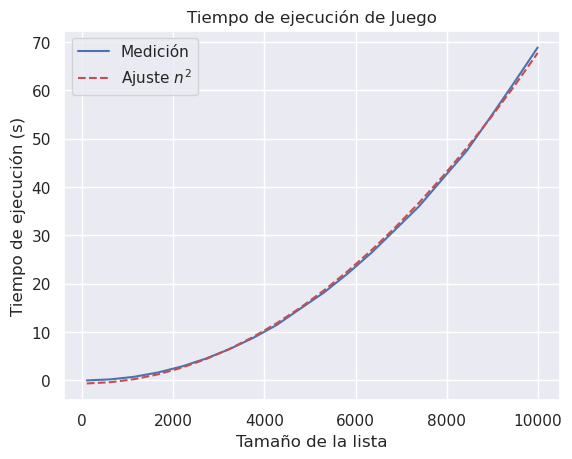
\includegraphics[width=0.60\textwidth]{images/Tiempo_y_ajuste.png}
	\caption{Tiempo de ejecución en función de la cantidad de elementos ($n$).}
	\label{fig:tiempo}
\end{figure}

Como se observa en la Figura \ref{fig:tiempo}, la medida presenta una superposición prácticamente exacta con la recta de ajuste de Cuadrados Mínimos\footnote{La técnica de Cuadrados Mínimos es un método de optimización matemática que, en este análisis, permite encontrar la función lineal que mejor se ajusta al conjunto de datos experimentales, \textit{minimizando} la suma de los errores al cuadrado entre los \textit{tiempos de ejecución} medidos y la recta $\mathcal{O}(n)$.}. Esto evidencia un comportamiento lineal respecto al incremento de elementos en el arreglo, confirmando que la complejidad temporal es $\mathcal{O}(n)$.


\begin{figure}[htbp]
    \centering
    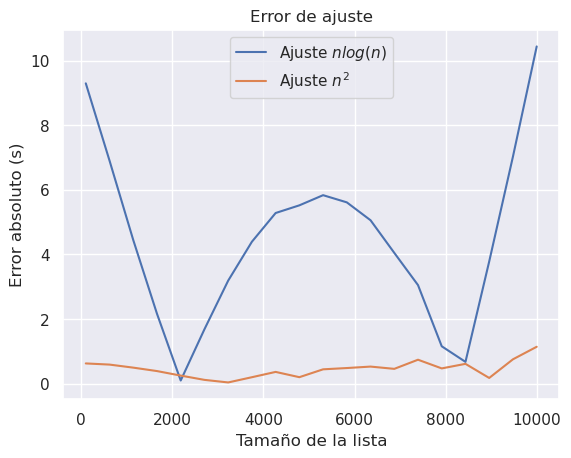
\includegraphics[width=0.60\textwidth]{images/Error_ajuste.png}
	\caption{Error absoluto del ajuste por Cuadrados Mínimos.}
	\label{fig:error}
\end{figure}

En la Figura \ref{fig:error} se refuerza el argumento, observando que el error absoluto se mantiene acotado y en magnitudes despreciables a lo largo de todo el rango de $n$, validando la complejidad temporal del algoritmo \textit{greedy} implementado.